Verwenden Sie die Greensche Funktion für das Interval $I=[-1,1]$,
um die Differentialgleichung
\begin{equation}
u''(x)=1-x^2
\label{70000006:dgl}
\end{equation}
auf $I$ mit Randbedingungen $u(-1)=u(1)=0$
zu lösen.

\begin{loesung}
In der Vorlesung wurde die Greensche Funktion für das Interval
$[0,1]$ konstruiert. Als erstes müssen wir daher die Greensche
Funktion für das Interval $[-1,1]$ anpassen. Dies kann auf
verschiedene Arten geschehen.
Einerseits kann man die Lösung aus dem
Skript nehmen, und durch Skalieren in die richtige Form bringen.
Man könnte auch einfach die Rechnung im Skript nochmals für
das Interval $[-1,1]$ durchführen. Drittens kann man
die Greensche Funktion aus singulänren Lösungen bestimmen.

In der Vorlesung wurde gezeigt, dass die Greensche Funktion
aus den partikulären Lösungen $\sigma(x,\xi)$ berechnet werden
kann.
Dazu muss man $\sigma(x,\xi)$ mit einer Lösung der homogenen Gleichung
ergänzen, so dass die Summe die Randbedingung erfüllt.
Im vorliegenden Fall ist also $u_r$ für
\[
G(x,\xi)=\sigma(x,\xi)+u_r(x,\xi)
=
{\textstyle\frac12}|x-\xi|+u_r(x,\xi)
\]
zu suchen, und $u_r$ muss eine Lösung der homogenen Gleichung sein.
In einer Dimension heisst das,
$u_r(x,\xi)=ax+b$, wobei $a$ und $b$ so zu bestimmen sind, dass die
Randbedingung erfüllt wird.
\begin{align*}
G(-1,\xi)&={\textstyle\frac12}|-1-\xi|-a+b&={\textstyle\frac12}(1+\xi)-a+b&=0\\
G(1,\xi)&={\textstyle\frac12}|1-\xi|+a+b&={\textstyle\frac12}(1-\xi)+a+b&=0
\end{align*}
Aus Summe und Differenz dieser beiden Gleichungen erhält man
schliesslich
\begin{align*}
1+2b&=0&\Rightarrow\qquad b&=-\frac12\\
\xi-2a&=0&\Rightarrow\qquad a&=\phantom{-}\frac{\xi}2
\end{align*}
Daraus folgt für die Greensche Funktion
\begin{align*}
G(x,\xi)
&=
{\textstyle\frac12}(|x-\xi|+x\xi-1)
\\
&=
\begin{cases}
{\textstyle\frac12}(x-\xi+x\xi - 1)
&\qquad x>\xi\\
{\textstyle\frac12}(\xi-x+x\xi - 1)
&\qquad x<\xi
\end{cases}
\end{align*}
Diese Form ist für die Berechnung der Lösung nicht optimal. Man kann
aber auch schreiben:
\begin{align*}
G(x,\xi)
&=
(x-\xi)\vartheta(x-\xi)-{\textstyle\frac12}(x+1)(1-\xi)
\\
&=
\begin{cases}
x-\xi
+
{\textstyle\frac12}(\xi-x+x\xi-1)
=
{\textstyle\frac12}(x-\xi+x\xi-1)
&\qquad x>\xi\\
{\textstyle\frac12}(\xi-x+x\xi-1)
&\qquad x<\xi
\end{cases}
\end{align*}
Damit ist die Greensche Funktion gefunden.

Mit dieser Greenschen Funktion kann jetzt die Lösung der
Differentialgleichung berechnet werden:
\begin{align*}
u(x)&=\int_{-1}^1
(x-\xi)\vartheta(x-\xi)-{\textstyle\frac12}(x+1)(1-\xi)
)(1-\xi^2)\,d\xi
\\
&=
\int_{-1}^1(x-\xi)\vartheta(x-\xi)(1-\xi^2)\,d\xi
-{\textstyle\frac12}(x+1)\int_{-1}^1(1-\xi)(1-\xi^2)\,d\xi
\\
&=
\int_{-1}^x(x-\xi)(1-\xi^2)\,d\xi
-{\textstyle\frac12}(x+1)\int_{-1}^1(1-\xi)(1-\xi^2)\,d\xi
\\
&=
-\frac1{12}(x^4-6x^2+5)
\end{align*}
wobei die Berechnung des Integrals mit Mathematica erfolgte.
Man kann durch Einsetzen nachprüfen, dass
$u(-1)=u(1)=0$ und dass $u''(x)=1-x^2$, die Greensche Funktion
liefert also tatsächlich eine Lösung des Problems.
\begin{figure}
\centering
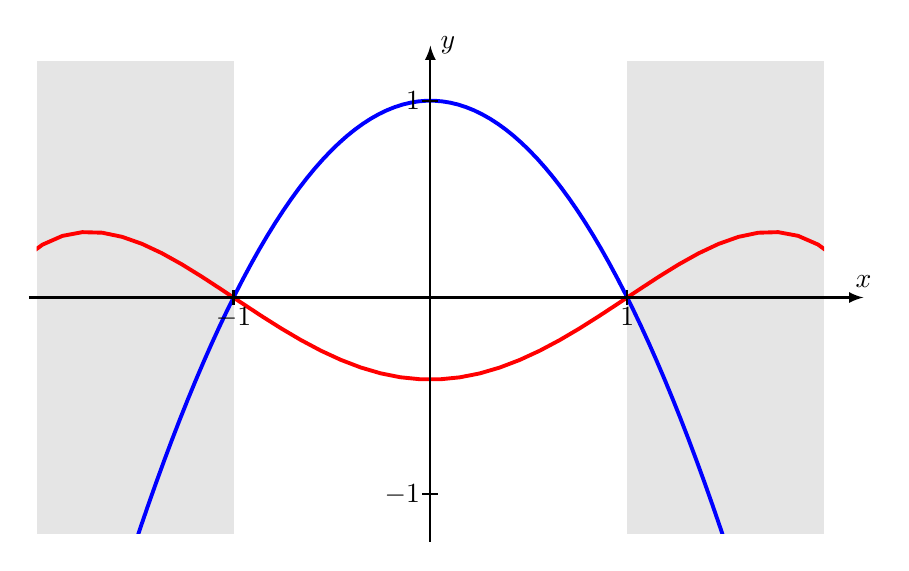
\begin{tikzpicture}[>=latex,thick]
\begin{scope}
\clip (-5,-3) rectangle (5,3);
\fill[color=gray!20] (-5,-3) rectangle (5,3);
\fill[color=white] (-2.5,-3.1) rectangle (2.5,3.1);
\draw[color=blue,line width=1.4pt]
	plot[domain=-2:2,samples=100]
		({2.5*\x},{2.5*(1-\x*\x)});
\draw[color=red,line width=1.4pt]
	plot[domain=-5:5,samples=100]
		({2.5*\x},{2.5*(-((\x*\x-6)*\x*\x+5)/12)});
\end{scope}
\draw[->] (-5.1,0) -- (5.5,0) coordinate[label={$x$}];
\draw[->] (0,-3.1) -- (0,3.2) coordinate[label={right:$y$}];
\draw (2.5,-0.1) -- (2.5,0.1);
\node at (2.5,0) [below] {$1$};
\draw (-2.5,-0.1) -- (-2.5,0.1);
\node at (-2.5,0) [below] {$-1$};
\draw (-0.1,-2.5) -- (0.1,-2.5);
\node at (0,-2.5) [left] {$-1$};
\draw (-0.1,2.5) -- (0.1,2.5);
\node at (0,2.5) [left] {$1$};
\end{tikzpicture}
\caption{Graph der Lösungsfunktion (rot) der Differentialgleichung
\ref{70000006:dgl}
mit homogenen Randbedingungen.
Die rechte Seite der Differentialgleichung ist in blau eingezeichnet.
Aus der Differentialgleichung~\eqref{70000006:dgl} folgt, dass die zweite
Ableitung an den Intervallenden verschwindet, die Lösung hat dort
also nicht nur eine Nullstelle sondern auch einen Wendepunkt.
\label{70000006:fig}}
\end{figure}

Nun noch die Berechnung der Greenschen Funktion als Skalierung
der bereits berechneten Funktion. Die Greensche Funktion $G(x,\xi)$ für
das Interval $[0,1]$
$G(x,\xi)$ hat die Eigenschaft, dass die partielle Funktion
$x\mapsto G(x,\xi)$ für jedes $\xi$ die Randbedingungen erfüllt,
und ausserdem
\[
\frac{\partial^2}{\partial x^2}G(x,\xi)=\delta(x-\xi).
\]
Der Ausdruck $\frac12(x+1)$ bildet $-1$ auf $0$ und $1$ auf $1$
ab, setzt man ihn in die Greensche Funktion $K(x,\xi)$ ein,
die für das Interval $[0,1]$ berechnet wurde,
erhält man eine Funktion
\[
G(x,\xi)=K({\textstyle\frac12}(x+1),{\textstyle\frac12}(\xi+1)),
\]
welche
für jeden Wert von $\xi$ die Randbedingung erfüllt, also
$K(\frac12(-1+1),\frac12(\xi+1))=G(0,\frac12(\xi+1))=0$ und
$G(\frac12(1+1),\frac12(\xi+1))=G(1,\frac12(\xi+1))=0$.
Die Bedingung, dass die zweite Ableitung eine Dirac-Distribution
sein muss, wird jedoch verletzt. Wir überlegen uns, wie die
die Skalierung den Wert der Ableitung verändert.
Die Ableitung von $G$ nach der ersten Variablen ist:
\begin{align*}
\frac{\partial}{\partial x}G(x,\xi)
&=
\frac{\partial}{\partial x}K({\textstyle\frac12}(x+1),{\textstyle\frac12}(\xi+1))\frac{\partial}{\partial x}\frac12(x+1)
=
\frac12\frac{\partial }{\partial x}K({\textstyle \frac12}(x+1), {\textstyle\frac12}(\xi+1))
\end{align*}
Die Funktion
\[
x\mapsto K(x,\xi)=\begin{cases}
(x-\xi)-x(1-\xi)=\xi(x-1)&\qquad x>\xi
\\
-x(1-\xi)&\qquad x<\xi
\end{cases}
\]
ist in jedem Teilinterval $x>\xi$ und $x<\xi$ eine lineare Funktion. Die Ableitung
ist also eine stückweise konstante Funktion.
Die Ableitung davon ist überall $0$, ausser an der Stelle $x=\xi$,
insbesondere ist die Ableitung der skalierten Ableitung gleich gross
wie die Ableitung der unskalierten Ableitung, der Faktor $\frac12$ ist
also alles, was kompensiert werden muss.

Die Greensche Funktion für dieses Problem wird damit
\begin{align*}
G(x,\xi)&=
2K({\textstyle\frac12}(x+1),{\textstyle\frac12}(\xi+1))
\\
&=
2
({\textstyle\frac12}(x+1)-\textstyle{\frac12}(\xi+1))
\vartheta({\textstyle\frac12}(x+1)-{\textstyle\frac12}(\xi+1))
-2{\textstyle\frac12}(x+1)(1-{\textstyle\frac12}(\xi+1))
\\
&=
(x-\xi)\vartheta(x-\xi)-{\textstyle\frac12}(x+1)(1-\xi).
\qedhere
\end{align*}
\end{loesung}
